% !TeX program = xelatex
\documentclass[10pt]{beamer}

\usetheme{metropolis}

\usepackage{pgfplots}
\usepgfplotslibrary{fillbetween}
\usepackage{pgfopts}
\usepackage{amsmath}
%\usepackage{structuralanalysis}
\usepackage{tikz}
\usepackage{tikz-3dplot}
\usepackage{chngcntr}
\usepackage{wasysym}
\usepackage{mathtools}
\usepackage{alphalph}
\usepackage{xcolor}
\usepackage[showdow=false, en-US]{datetime2}
\usepackage{hyperref}

\newcommand{\highlight}[1]{%
	\colorbox{red!50}{$\displaystyle#1$}}

\setcounter{lecture}{26}
\counterwithin{equation}{lecture}
\makeatletter
\def\user@resume{resume}
\def\user@intermezzo{intermezzo}
%
\newcounter{previousequation}
\newcounter{lastsubequation}
\newcounter{savedparentequation}
\setcounter{savedparentequation}{1}
% 
\renewenvironment{subequations}[1][]{%
	\def\user@decides{#1}%
	\setcounter{previousequation}{\value{equation}}%
	\ifx\user@decides\user@resume 
	\setcounter{equation}{\value{savedparentequation}}%
	\else  
	\ifx\user@decides\user@intermezzo
	\refstepcounter{equation}%
	\else
	\setcounter{lastsubequation}{0}%
	\refstepcounter{equation}%
	\fi\fi
	\protected@edef\theHparentequation{%
		\@ifundefined {theHequation}\theequation \theHequation}%
	\protected@edef\theparentequation{\theequation}%
	\setcounter{parentequation}{\value{equation}}%
	\ifx\user@decides\user@resume 
	\setcounter{equation}{\value{lastsubequation}}%
	\else
	\setcounter{equation}{0}%
	\fi
	\def\theequation  {\theparentequation  \alph{equation}}%
	\def\theHequation {\theHparentequation \alph{equation}}%
	\ignorespaces
}{%
%  \arabic{equation};\arabic{savedparentequation};\arabic{lastsubequation}
\ifx\user@decides\user@resume
\setcounter{lastsubequation}{\value{equation}}%
\setcounter{equation}{\value{previousequation}}%
\else
\ifx\user@decides\user@intermezzo
\setcounter{equation}{\value{parentequation}}%
\else
\setcounter{lastsubequation}{\value{equation}}%
\setcounter{savedparentequation}{\value{parentequation}}%
\setcounter{equation}{\value{parentequation}}%
\fi\fi
%  \arabic{equation};\arabic{savedparentequation};\arabic{lastsubequation}
\ignorespacesafterend
}
\makeatother
\title{AE 737 - Mechanics of Damage Tolerance}
\subtitle{Lecture \arabic{lecture}}
\date{Last Updated: \today\ at \DTMcurrenttime}
\author{Dr. Nicholas Smith}
\institute{Wichita State University, Department of Aerospace Engineering}
% \titlegraphic{\hfill\includegraphics[height=1.5cm]{logo/logo}}

\begin{document}
	
	\maketitle
	\begin{frame}{schedule}
		\begin{itemize}
			\item 5 May - Repair, NDT
			\item 10 May - Final Project Due by 5:00 pm
		\end{itemize}
	\end{frame}
	
	\begin{frame}{skunk works talk}
		\begin{columns}
			\begin{column}{0.45\linewidth}
			\begin{itemize}
				\item Friday, May 6
				\item 12:00 - 1:00 pm
				\item Shocker Hall Multipurpose Room - Honors College
				\item Pizza (first-come first-served)
			\end{itemize}
			\end{column}
			\begin{column}{0.45\linewidth}
				\begin{figure}
				\centering
				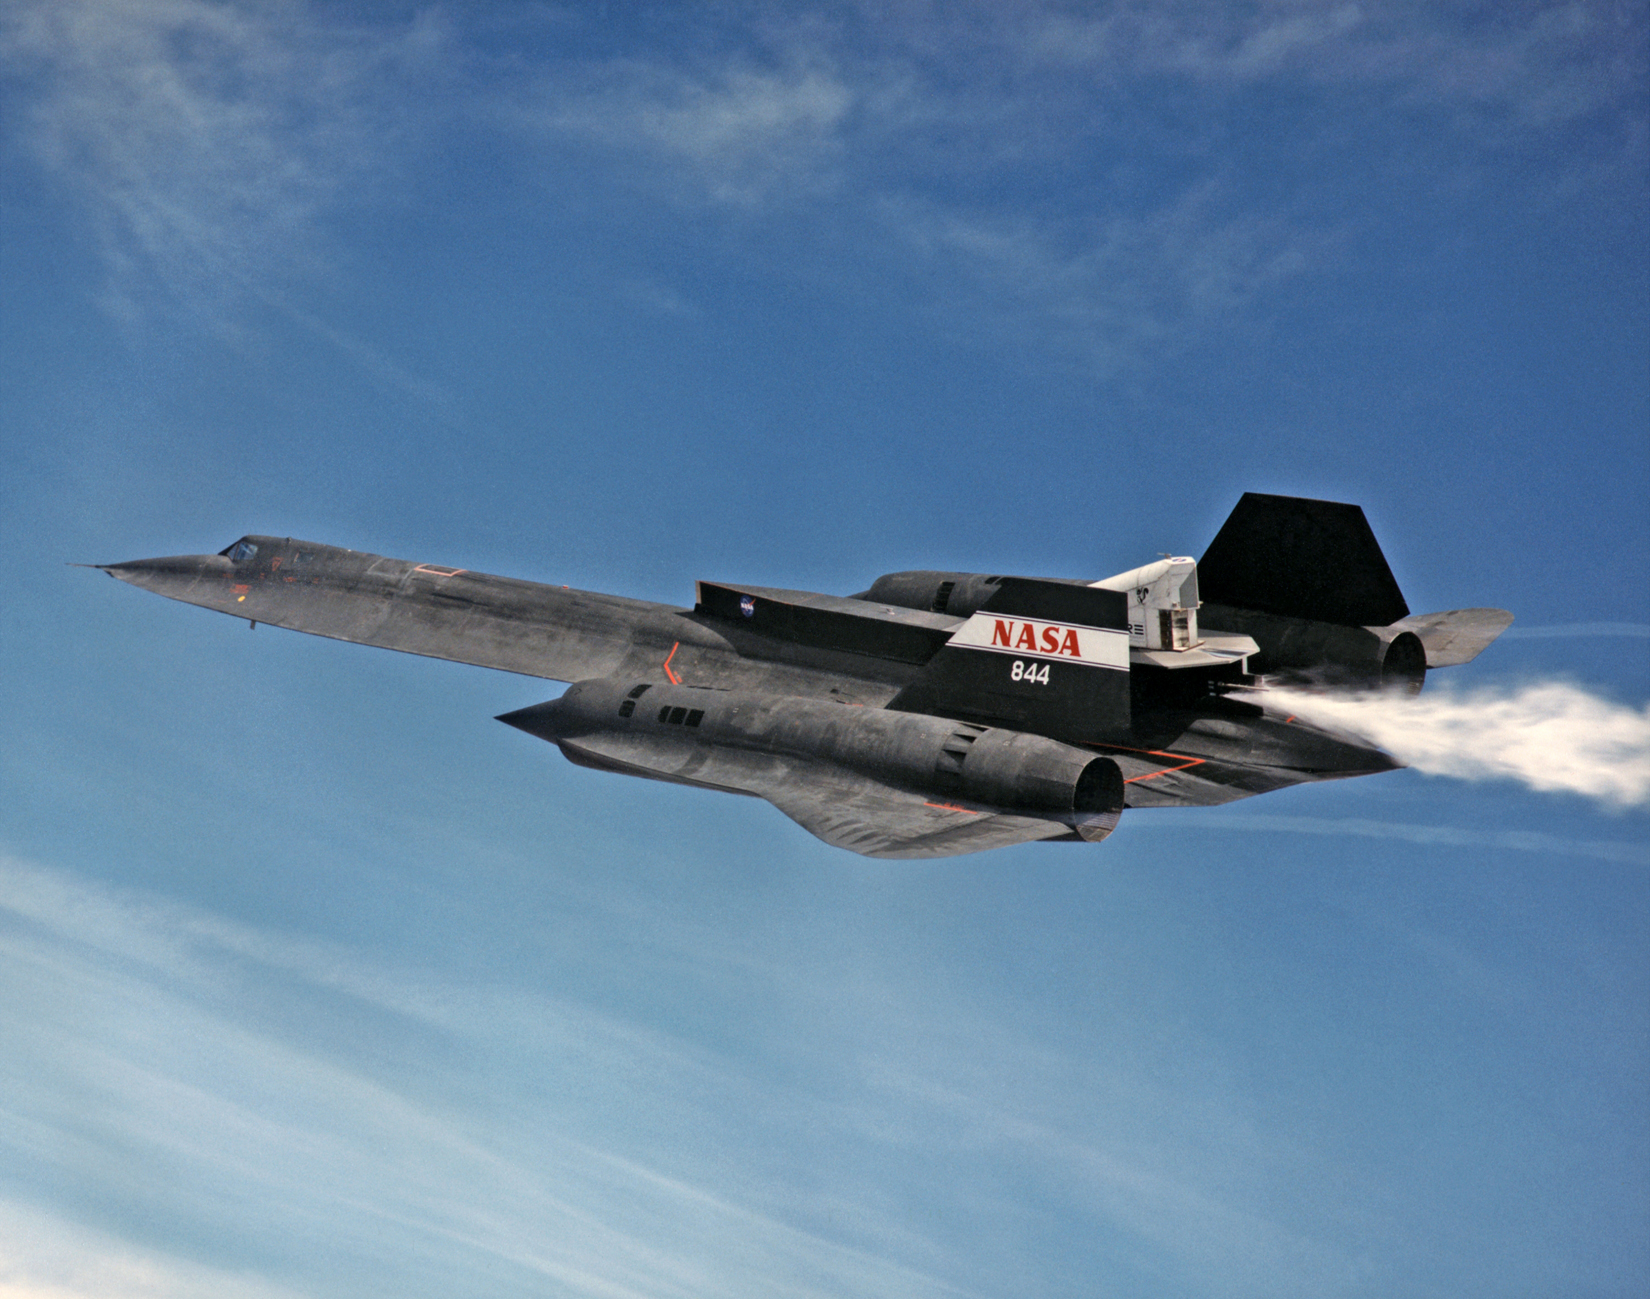
\includegraphics[width=0.7\linewidth]{../Figures/SR-71_LASRE_cold_test}
				\caption{LASRE on top of SR-71 Blackbird}
				\label{fig:SR-71_LASRE_cold_test}
				\end{figure}
			\end{column}
		\end{columns}
	\end{frame}
	
	\begin{frame}
		\frametitle{outline}
		\setbeamertemplate{section in toc}[sections numbered]
		\tableofcontents[hideallsubsections]
	\end{frame}

	\section{repairing cracked structures}
	
	\begin{frame}{repair}
		\begin{itemize}[<+->]
			\item Depending on the location and severity of damage, there are a few options for repair
			\item Replacement
			\item Stop drilling
			\item Welding
			\item Patching
			\item Oversize fasteners
			\item Load Reduction/improved analysis
			\item Residual stresses
		\end{itemize}
	\end{frame}
	
	\begin{frame}{stop drilling}
		\begin{itemize}[<+->]
			\item If a crack is not of dangerous length, full repair/replacement is not necessary
			\item Stop drilling refers to a hole drilled at the crack tip
			\item This hole removes the crack tip, crack will re-initiate at edge of hole
			\item Still susceptible to MSD in future
			\item Some new techniques attempt to change direction of crack growth
		\end{itemize}
	\end{frame}
	
	\begin{frame}{welding}
		\begin{itemize}[<+->]
			\item Crack material is machined away
			\item Empty space is filled with weld
			\item Can cause distortion
			\item Sometimes heat treatment is needed
		\end{itemize}
	\end{frame}
	
	\begin{frame}{patching}
		\begin{itemize}[<+->]
			\item A patch placed over the crack provides an alternate load path
			\item Patches can be attached mechanically, with fasteners
			\item Or bonded with adhesives
			\item Fasteners introduce new holes, new sites for damage
			\item Additional fasteners add weight
			\item Adhesives add less weight, do not introduce new damage, but it can be difficult to ensure the integrity of the bond in-service
		\end{itemize}
	\end{frame}
	
	\begin{frame}{oversize fastener}
		\begin{itemize}[<+->]
			\item When crack forms around a fastener hole, the hole can be drilled larger
			\item The larger hole removes the crack tip
			\item Fastener is replaced with a larger fastener, appropriate to the drilled hole
		\end{itemize}
	\end{frame}
	
	\begin{frame}{load reduction}
		\begin{itemize}[<+->]
			\item When damaged parts are difficult or expensive to repair, load can be reduced instead
			\item (e.g. assign a plane to a less rigorous flight path)
			\item Initial designs are often conservative
			\item After years of life, more advanced analysis is usually available
			\item Sometimes repair and load reduction are not necessary if initial design is found to be overly conservative
		\end{itemize}
	\end{frame}
	
	\begin{frame}{residual stress}
		\begin{itemize}[<+->]
			\item Some repair methods introduce beneficial residual stresses instead of directly addressing the crack
			\item Surface treatments can introduce compressive residual stresses at the crack tip, which can slow or stop crack growth
			\item Some common methods used are
			\item Shot peening
			\item Low plasticity burnishing
			\item Laser shock peening
			\item Hole cold-working
		\end{itemize}
	\end{frame}
	
	\begin{frame}{shot peening}
		\begin{figure}
		\centering
		\includegraphics[width=0.7\linewidth]{"../Figures/shot-peening"}
		\end{figure}
	\end{frame}
	
	\begin{frame}{hole cold working}
		\begin{figure}
		\centering
		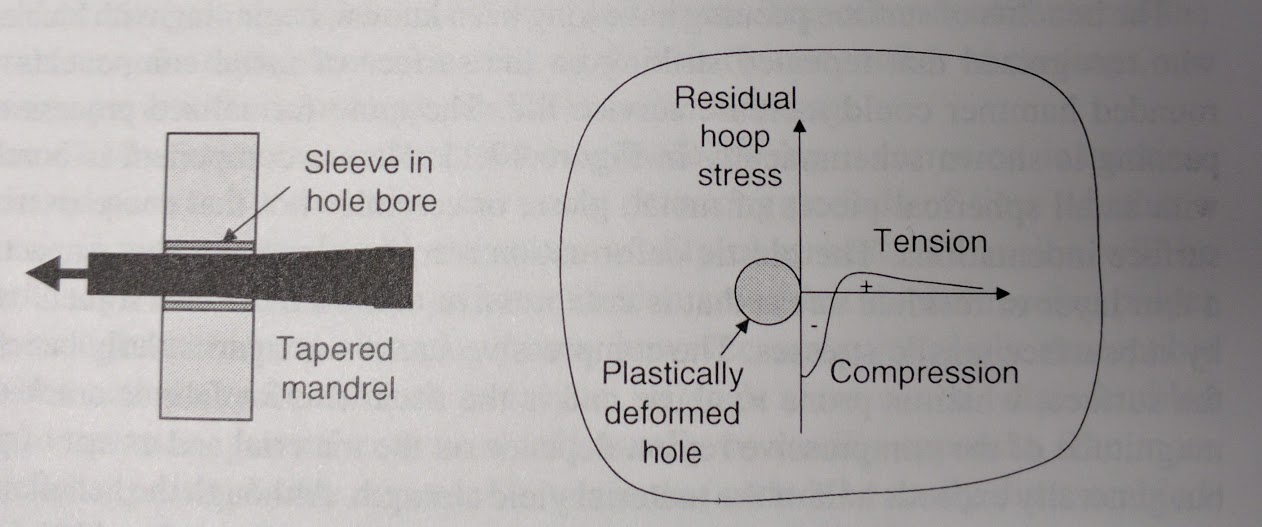
\includegraphics[width=0.7\linewidth]{../Figures/hole-cold-working}
		\end{figure}
	\end{frame}
	
	\begin{frame}{hole cold working}
		\begin{figure}
		\centering
		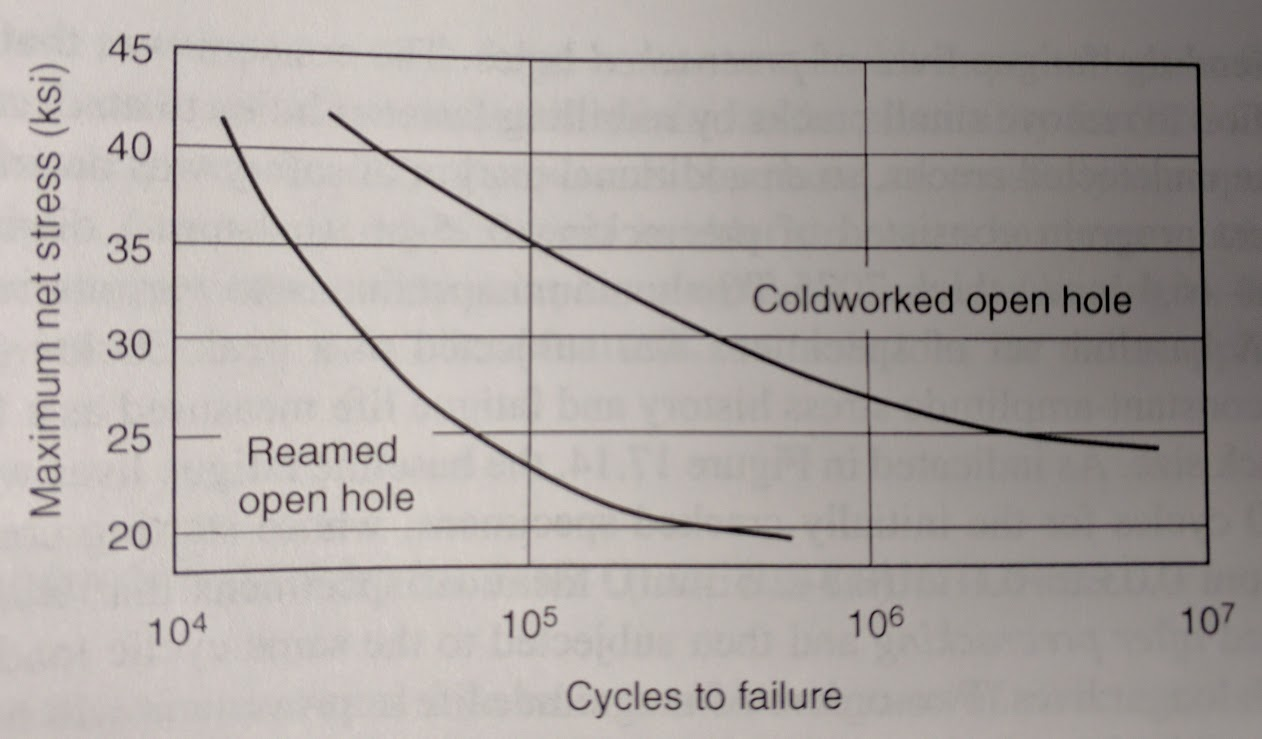
\includegraphics[width=0.7\linewidth]{../Figures/hole-SN}
		\end{figure}
	\end{frame}
	
	\begin{frame}{which repair method}
		\begin{itemize}[<+->]
			\item Which repair method is best?
			\item Factors that affect decision
			\item Cost
			\item Is multiple site damage a concern?
			\item Fracture vs. net section yield
			\item Can we reduce $K_{max}$ below $K_{th}$ with residual stresses?
		\end{itemize}
	\end{frame}
	
	\section{group problems}
	
	\begin{frame}{group 1}
		\begin{columns}
			\begin{column}{0.48\linewidth}
				\begin{itemize}
					\item Compare the effectiveness of stop drilling in 2024 and 7075 for the following panel.
					\item For 2024 use $K_c = 125 \text{ ksi}\sqrt{\text{in}}$ and $\sigma_{YS} = 50 \text{ ksi}$
					\item For 7075 use $K_c = 60 \text{ ksi}\sqrt{\text{in}}$ and $\sigma_{YS} = 70 \text{ ksi}$
					\item Recall $\beta = \sqrt{\sec(\pi a/W)}$
				\end{itemize}
			\end{column}
			
			\begin{column}{0.48\linewidth}
				\begin{figure}[H]
					\centering
					\begin{tikzpicture}
					\begin{scope}[scale=1.5]
					\draw (0,0) -- (0,1) -- (2,1) -- (2,-1) -- (0,-1) -- (0,0);
					\draw (0.8,0) -- (1.2,0);
					\draw node at (1,0.2) {2};
					\draw[->] (1,1) -- (1,1.5) node[above] {$\sigma$};
					\draw[->] (1,-1) -- (1,-1.5) node[below] {$\sigma$};
					\draw[->] (0.7,-0.7) -- (0,-0.7);
					\draw[->] (1.3,-0.7) -- (2,-0.7);
					\draw node at (1,-0.7) {$6$};
					\end{scope}
					\end{tikzpicture}
				\end{figure}
			\end{column}
		\end{columns}
	\end{frame}
	
	\begin{frame}{group 2}
		\begin{itemize}
			\item Due to MSD concerns, we would like to alter a crack path by $15^\circ$.
			\item What stresses would need to be added to a 15 ksi tensile load to accomplish this? 
			\item Note: Assume for this problem that $\beta^\prime = \beta$
			\item Recall
			\begin{align*}
			K_{II} &= \tau \sqrt{\pi a}\beta^\prime\\
			K_I \sin \theta_p + K_{II}\left(3\cos \theta_p -1 \right) &= 0
			\end{align*}
		\end{itemize}
	\end{frame}
	
	\begin{frame}{group 3}
		\begin{columns}
			\begin{column}{0.48\linewidth}
				\begin{itemize}
					\item Compare the amount of residual compressive stress needed stop crack growth for Al 2024 and Al 7075 in the following panel.
					\item Assume $K_{th} = 4 \text{ ksi}\sqrt{\text{in}}$ for Al 2024
					\item And $K_{th} = 7 \text{ ksi}\sqrt{\text{in}}$ for Al 7075
				\end{itemize}
			\end{column}
			
			\begin{column}{0.48\linewidth}
				\begin{figure}[H]
					\centering
					\begin{tikzpicture}
					\begin{scope}[scale=1.5]
					\draw (0,0) -- (0,1) -- (2,1) -- (2,-1) -- (0,-1) -- (0,0);
					\draw (0.8,0) -- (1.2,0);
					\draw node at (1,0.2) {0.5};
					\draw[->] (1,1) -- (1,1.5) node[above] {$20$};
					\draw[->] (1,-1) -- (1,-1.5) node[below] {$20$};
					\draw[->] (0.7,-0.7) -- (0,-0.7);
					\draw[->] (1.3,-0.7) -- (2,-0.7);
					\draw node at (1,-0.7) {$5$};
					\end{scope}
					\end{tikzpicture}
				\end{figure}
			\end{column}
		\end{columns}
		
	\end{frame}
	
	\begin{frame}{group 4}
		
			\begin{columns}
				\begin{column}{0.48\linewidth}
					\begin{itemize}
						\item Due to damage, an airline decides to move an aircraft to a less strenuous flight cycle. 
						\item Find the effective load for a flight cycle that will last at least 1000 flights for the following cracked panel.
						\item Note: use $p=4$ and $M_t = 25.8$
						\item Assume $K_c = 60 \text{ ksi}\sqrt{\text{in}}$ and $\sigma_{YS} = 70 \text{ ksi}$
						\item The largest load of 20 ksi occurs during takeoff and will not change with flight cycle.
					\end{itemize}
				\end{column}
				
				\begin{column}{0.48\linewidth}
					\begin{figure}[H]
						\centering
						\begin{tikzpicture}
						\begin{scope}[scale=1.5]
						\draw (0,0) -- (0,1) -- (2,1) -- (2,-1) -- (0,-1) -- (0,0);
						\draw (0.8,0) -- (1.2,0);
						\draw node at (1,0.2) {1.5};
						\draw[->] (1,1) -- (1,1.5) node[above] {$\sigma$};
						\draw[->] (1,-1) -- (1,-1.5) node[below] {$\sigma$};
						\draw[->] (0.7,-0.7) -- (0,-0.7);
						\draw[->] (1.3,-0.7) -- (2,-0.7);
						\draw node at (1,-0.7) {$7$};
						\end{scope}
						\end{tikzpicture}
					\end{figure}
				\end{column}
			\end{columns}
	\end{frame}
	
\end{document}
